\documentclass[11pt]{amsart}
\input{glyphtounicode}
\pdfgentounicode=1

\usepackage[T1]{fontenc}
\usepackage[utf8]{inputenc}
\usepackage{amsmath,amssymb}
\usepackage{graphicx}
\usepackage{geometry}
\usepackage{xcolor}
\usepackage{hyperref}
\geometry{margin=1in}
\sloppy
\graphicspath{{figures/}}
\hypersetup{
  colorlinks=true,
  linkcolor=blue!45!black,
  pdftitle={Spectral A-N v18: Supplementary Visual Atlas},
  pdfauthor={Eliuth Chavero Jasso}
}

\title[Spectral A-N v18: Supplementary Visual Atlas]{Spectral A-N v18: Supplementary Visual Atlas}
\author{Eliuth Chavero Jasso}
\address{Independent Researcher, Apizaco, Tlaxcala, Mexico}
\date{30 July 2026}

\begin{document}
\maketitle

\begin{abstract}
Nine figures generated directly from this pass's executed experiment
artifacts (\texttt{generate\_figures.py}, colorblind-safe Okabe--Ito
palette throughout). Figures 1--7 cover the highest-value single-
configuration results from the accompanying certification paper; Figures
8--9 (new, from a follow-up 416-cell hardware sweep) directly close two
of the gaps the original version of this atlas listed as missing ---
associator-ratio behavior across a swept grid, and CPU/GPU parity across
multiple dimensions rather than one. This remains a focused atlas, not
the full twenty-figure set the original mission brief enumerates; what is
still NOT included is listed explicitly in Section~\ref{sec:missing}
rather than silently omitted.
\end{abstract}

\section{Figures}

\begin{figure}[h]
\centering
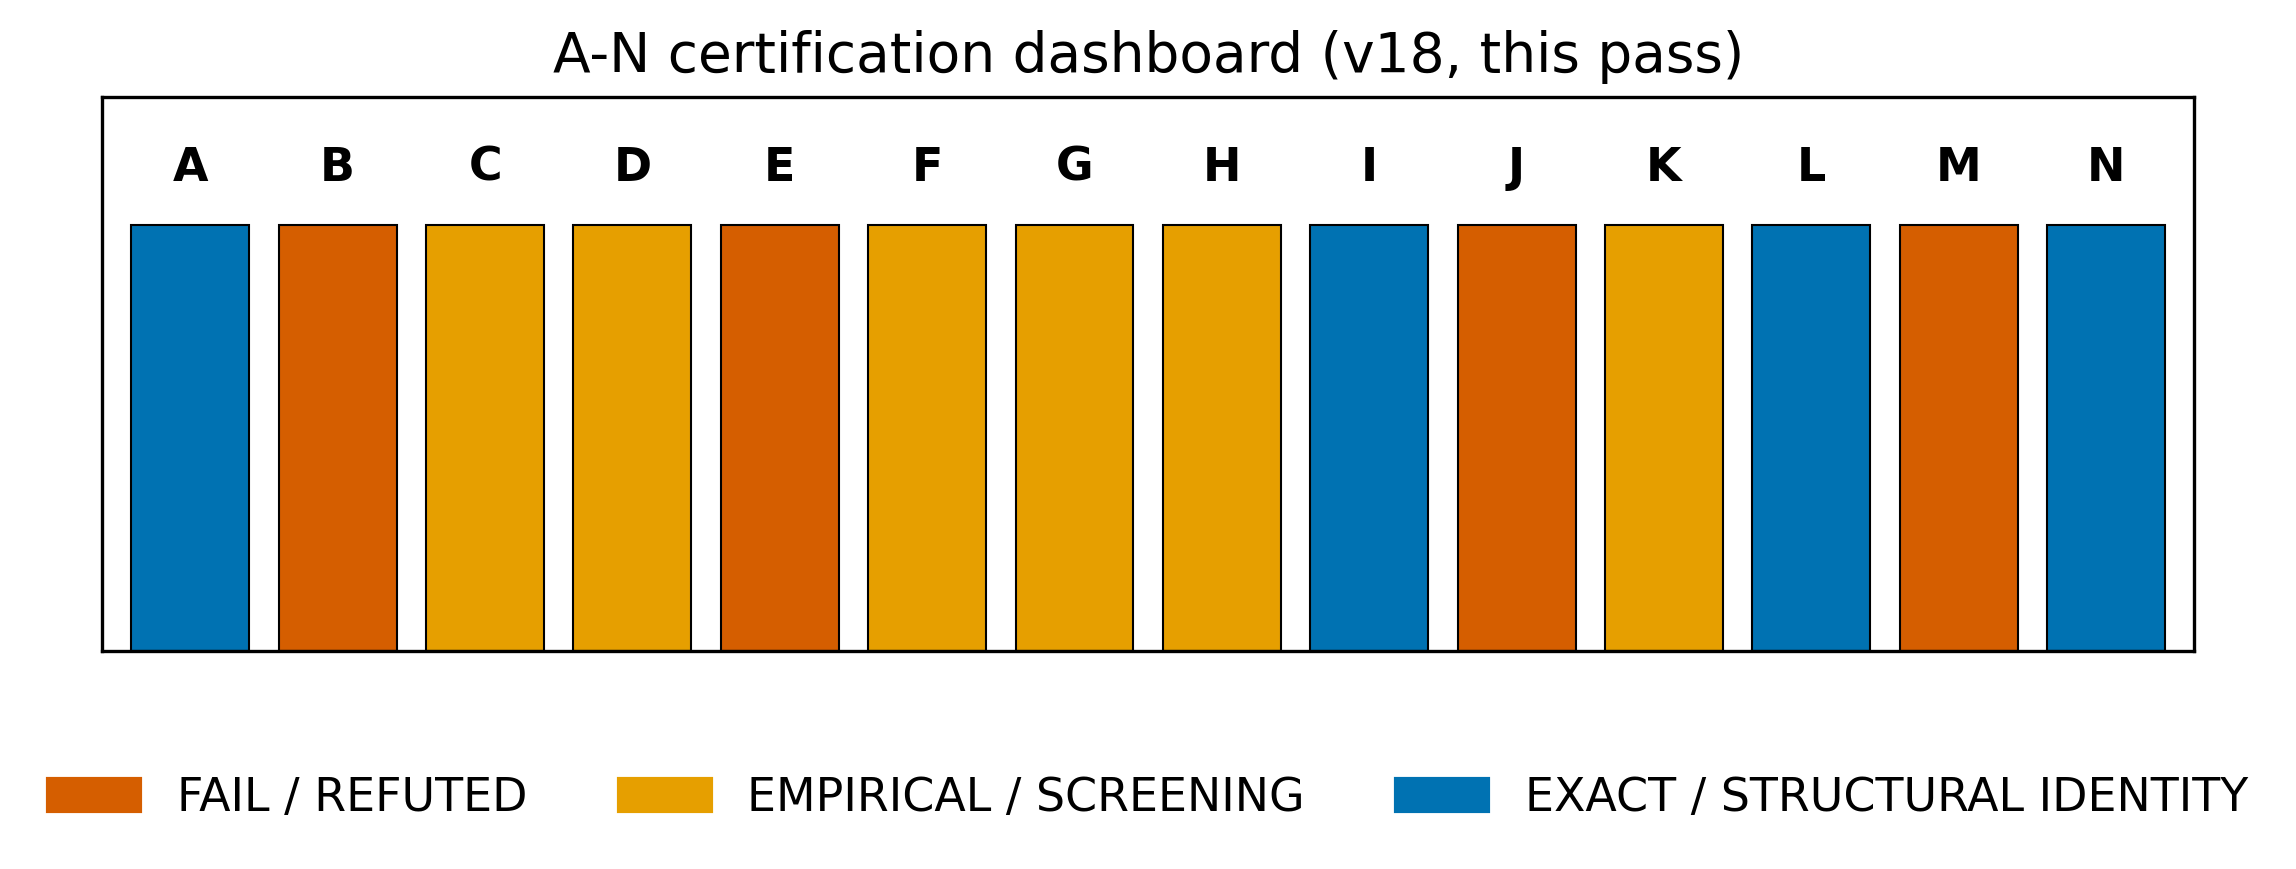
\includegraphics[width=0.85\textwidth]{01_an_dashboard}
\caption{A-N certification dashboard. Blue = exact/structural-identity
component present; orange = empirical/screening-only evidence; vermillion
= fail/refuted for the scientific claim. Every block carries at least one
structural or empirical component; the vermillion blocks (B, E, J, M) are
where the scientific (non-structural) claim specifically failed.}
\end{figure}

\begin{figure}[h]
\centering
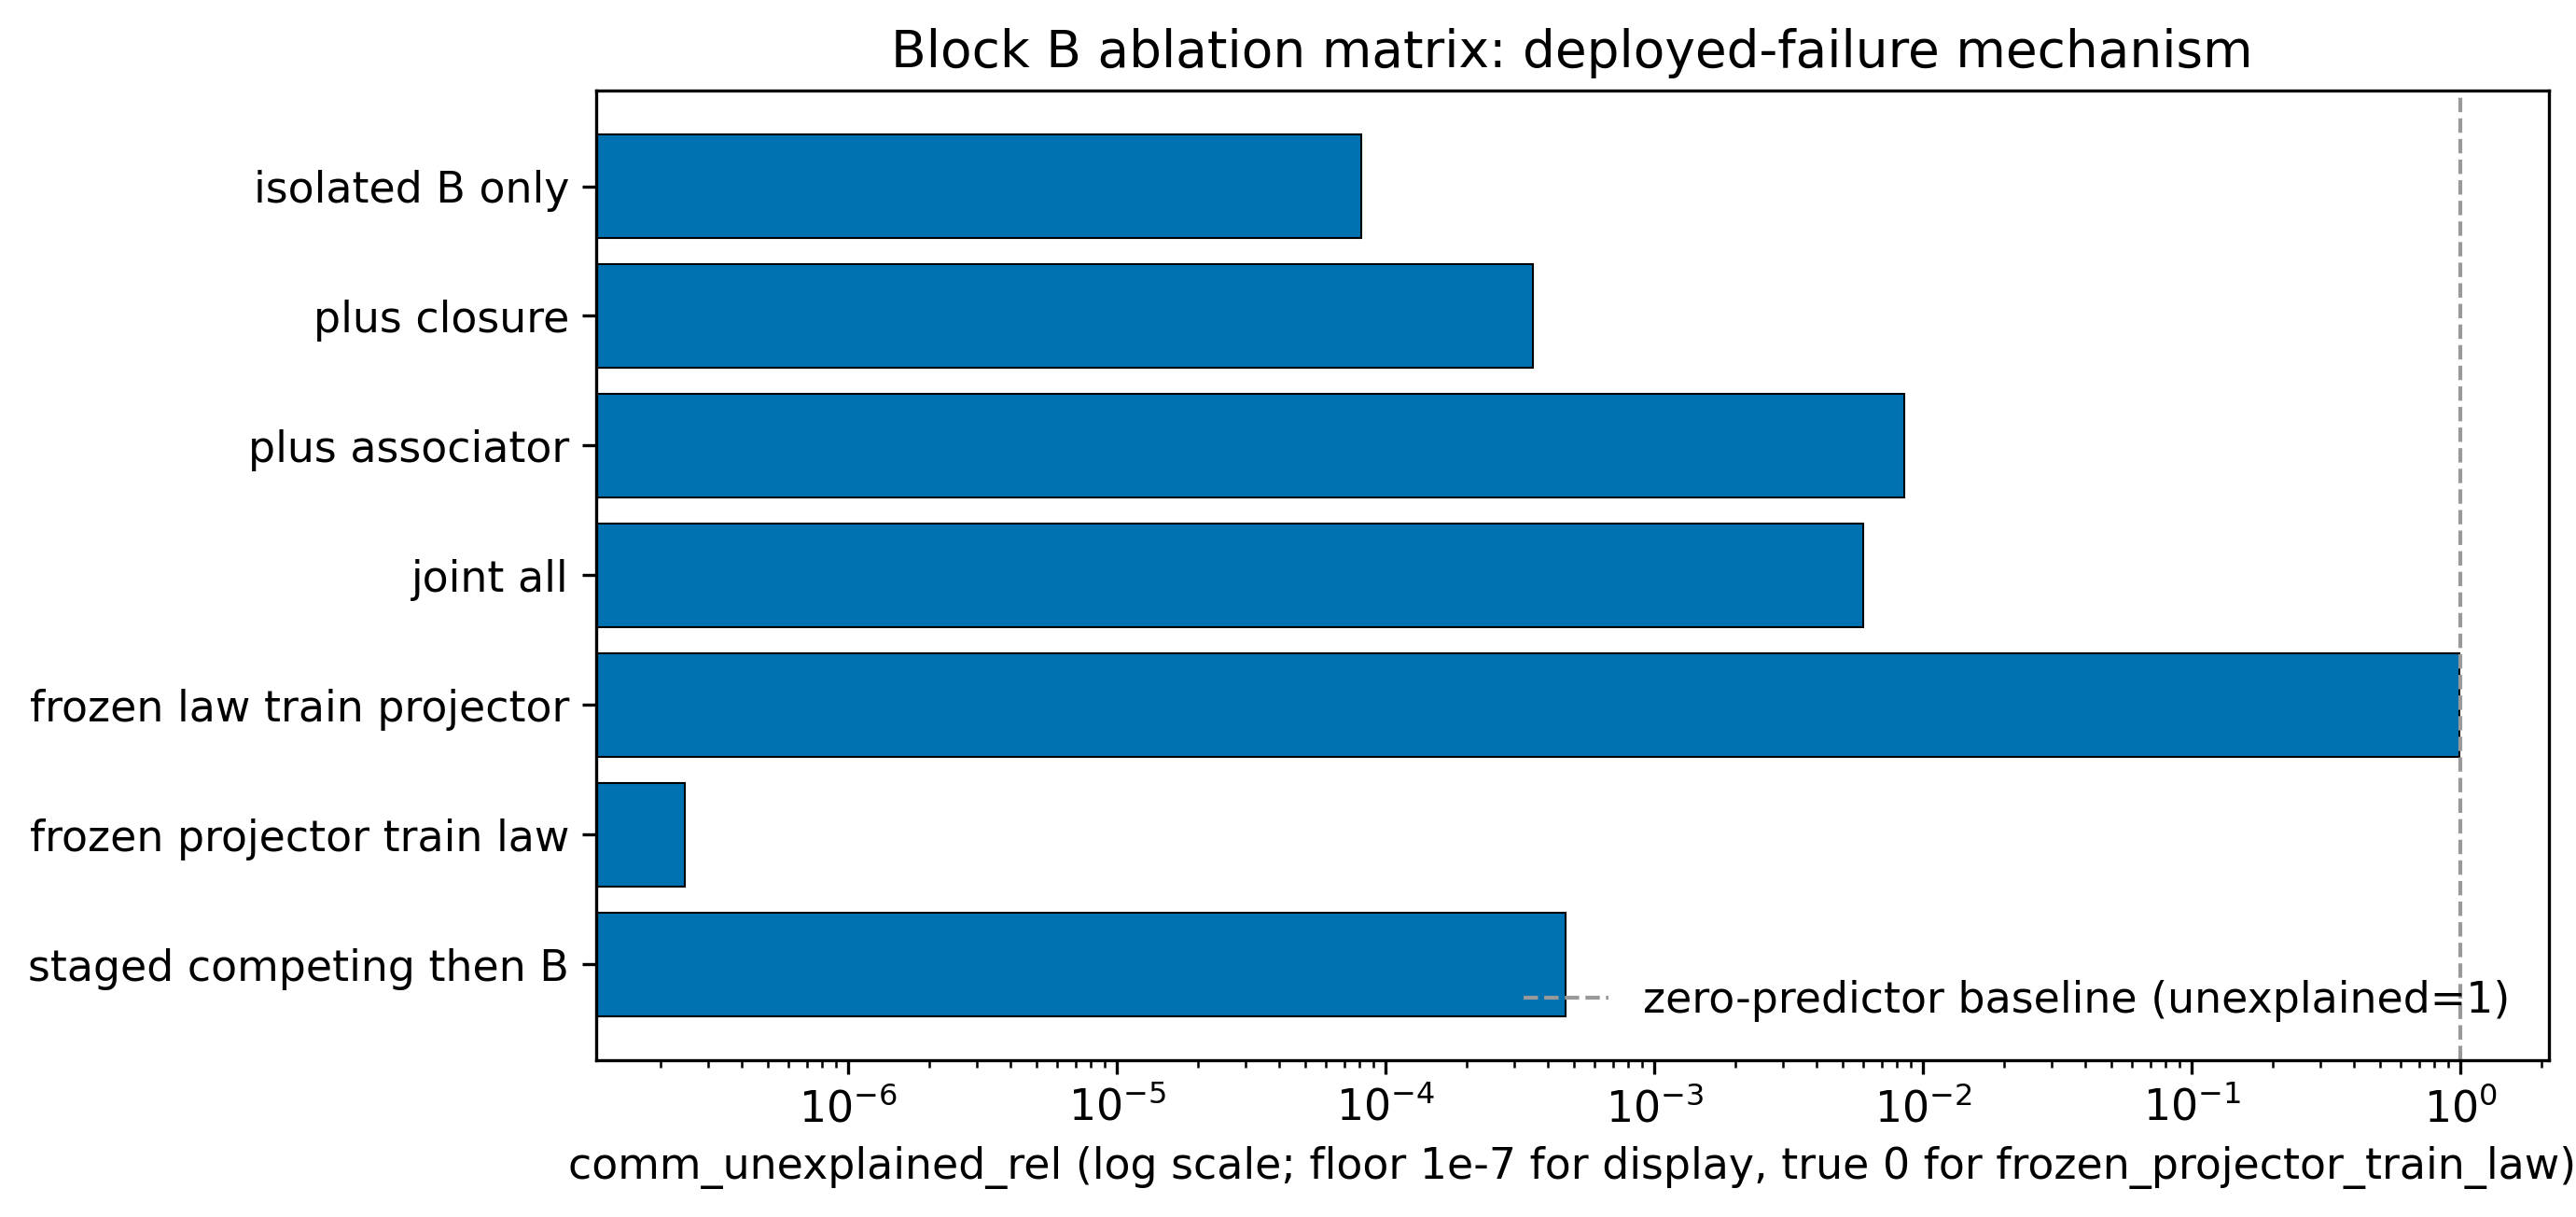
\includegraphics[width=0.9\textwidth]{02_block_b_ablation}
\caption{Block B ablation matrix. The dashed line marks the trivial
zero-predictor baseline. Note \texttt{frozen\_projector\_train\_law}
reaches exactly zero (displayed at the floor for the log axis) while
\texttt{frozen\_law\_train\_projector} barely moves off the zero-predictor
line --- the explanatory power lives in the law's parameters, not the
learned subspace.}
\end{figure}

\begin{figure}[h]
\centering
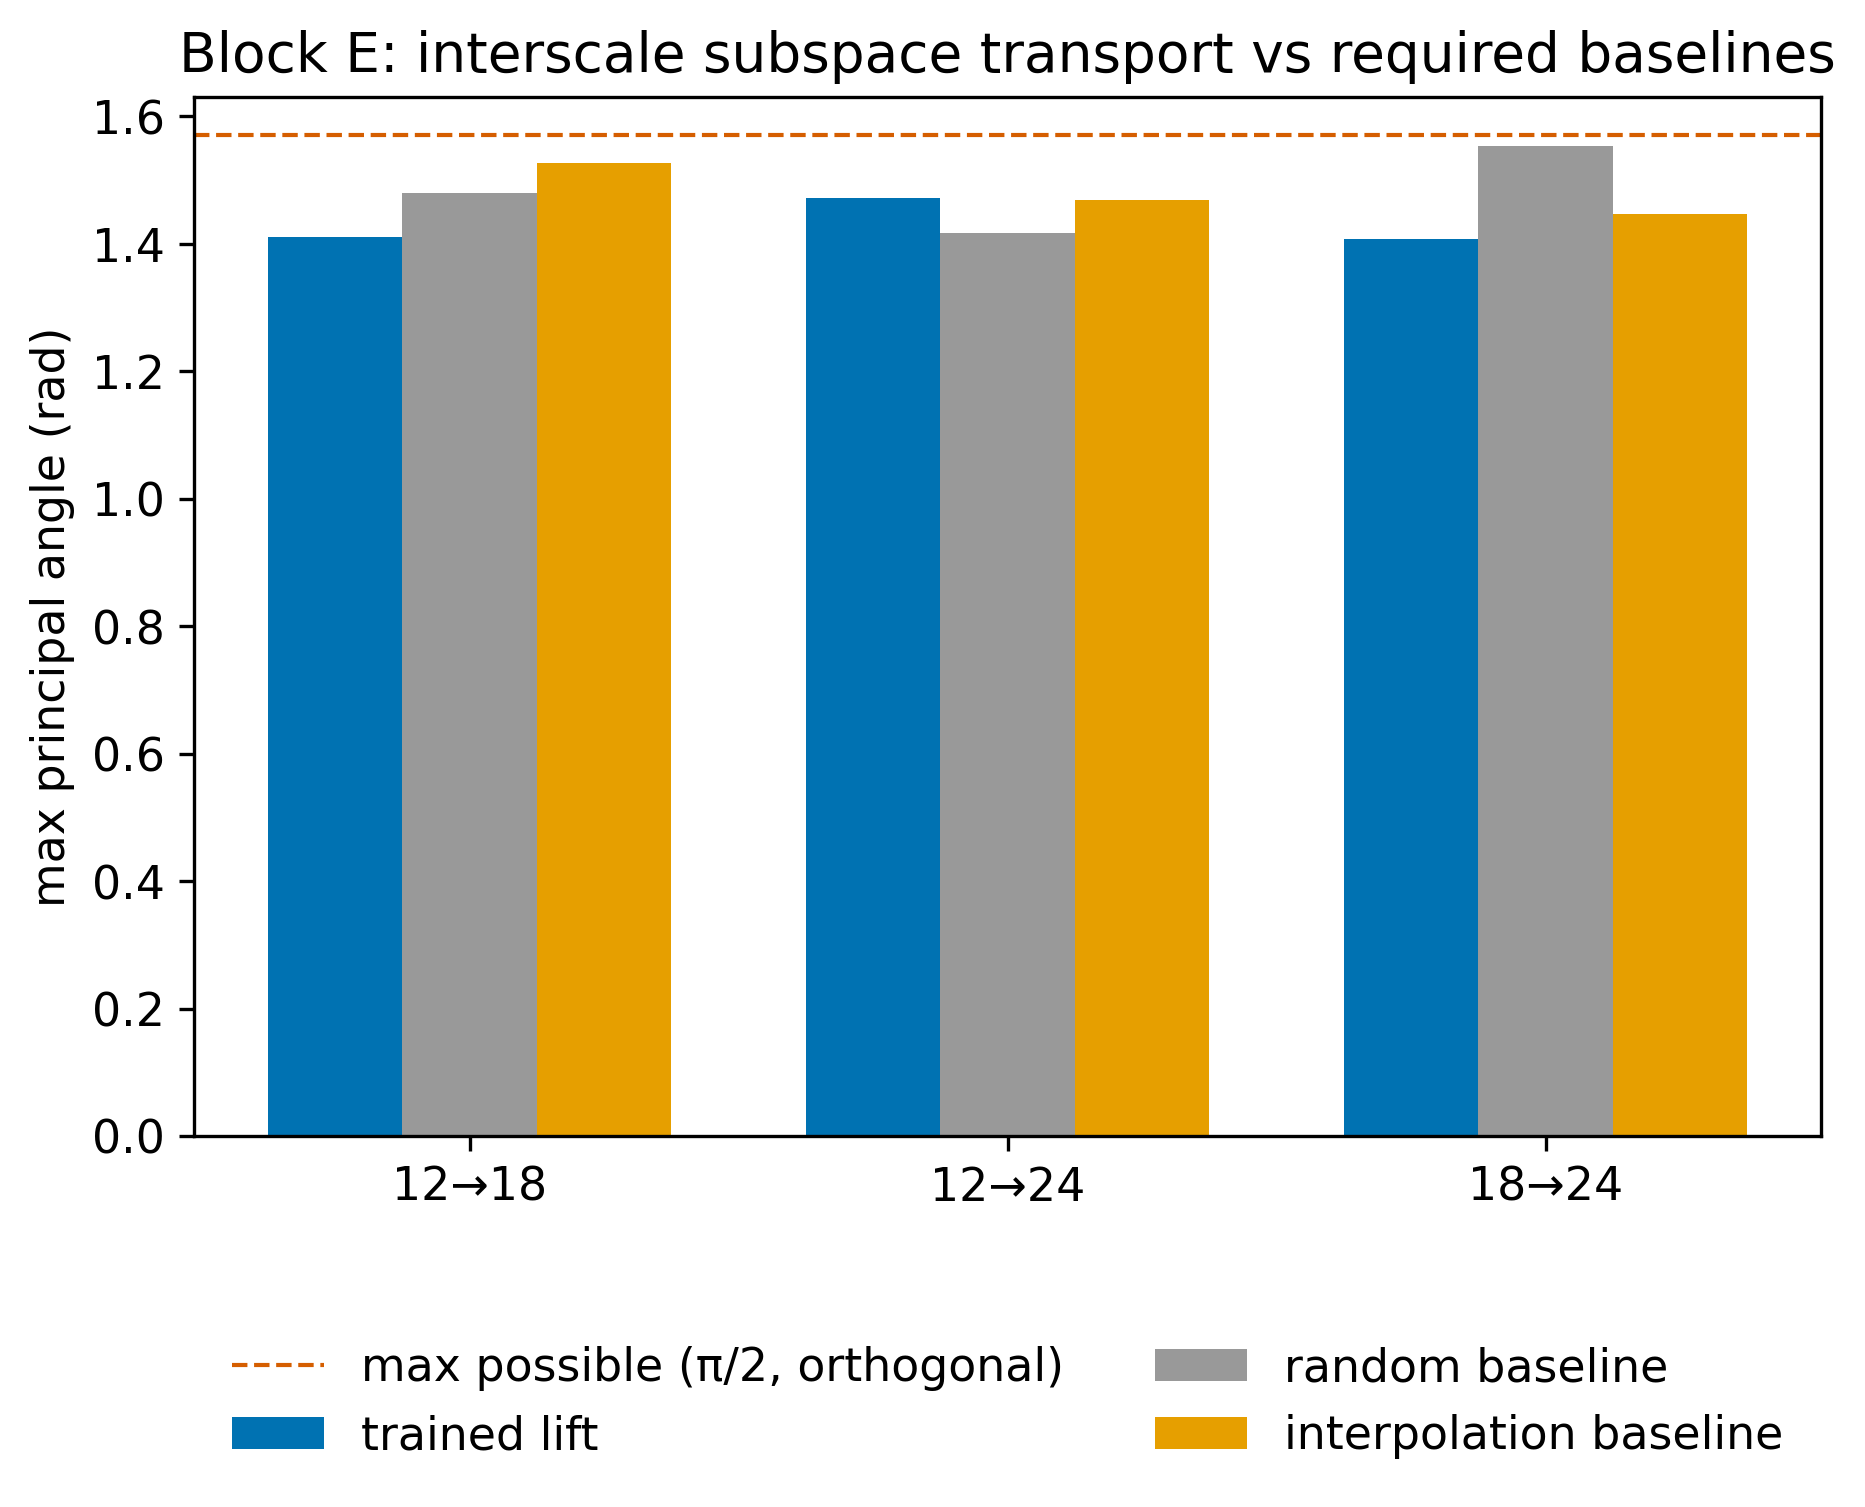
\includegraphics[width=0.85\textwidth]{03_block_e_transport}
\caption{Block E interscale transport: all three conditions (trained
lift, random-subspace baseline, interpolation baseline) sit close to the
maximum possible angle ($\pi/2$, complete orthogonality) for every
resolution pair --- the visual signature of ``no real transport signal,''
not merely a numerically small effect size.}
\end{figure}

\begin{figure}[h]
\centering
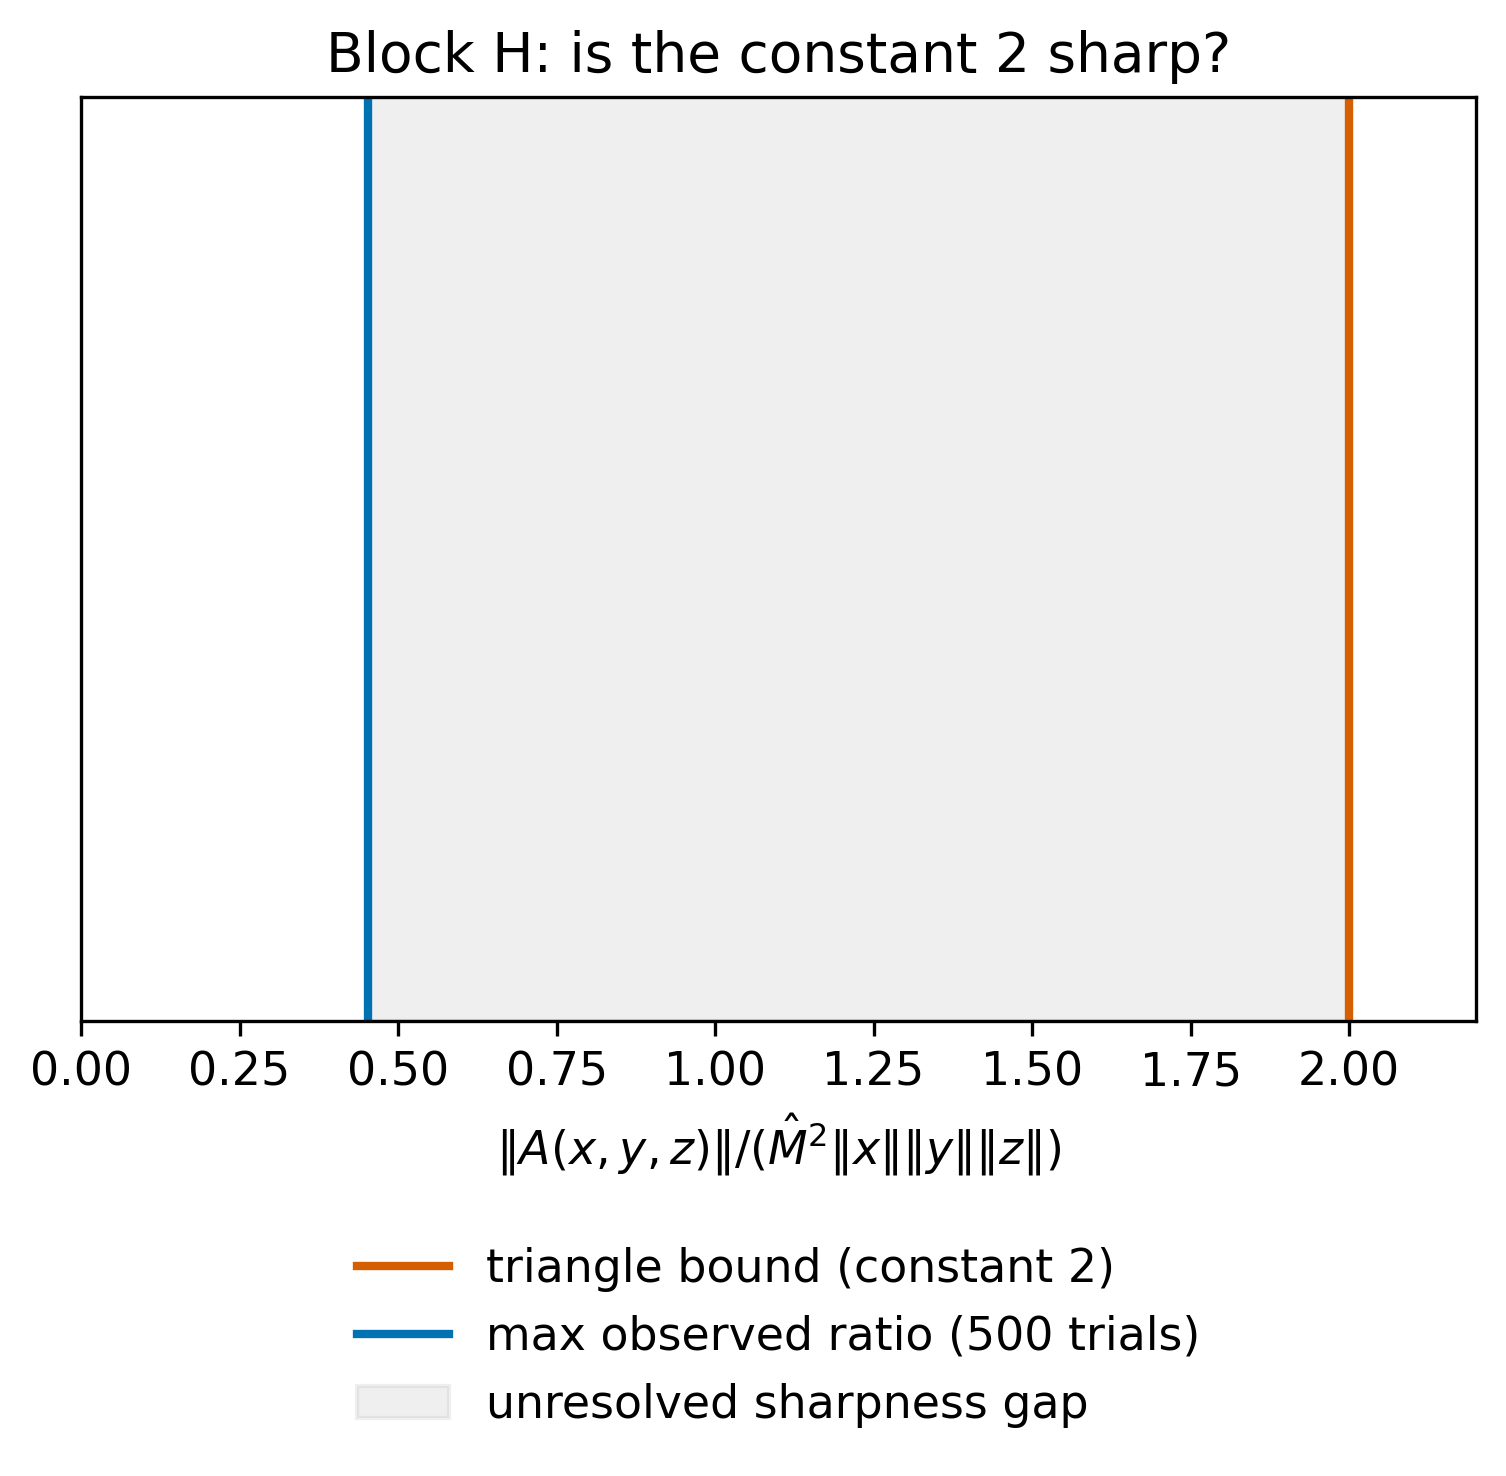
\includegraphics[width=0.7\textwidth]{04_block_h_sharpness}
\caption{Block H: the shaded region is the unresolved gap between the
proved upper bound (2) and the best adversarially-found ratio (0.452).
Sharpness of the constant 2 remains open; the gap is large, not a
near-miss.}
\end{figure}

\begin{figure}[h]
\centering
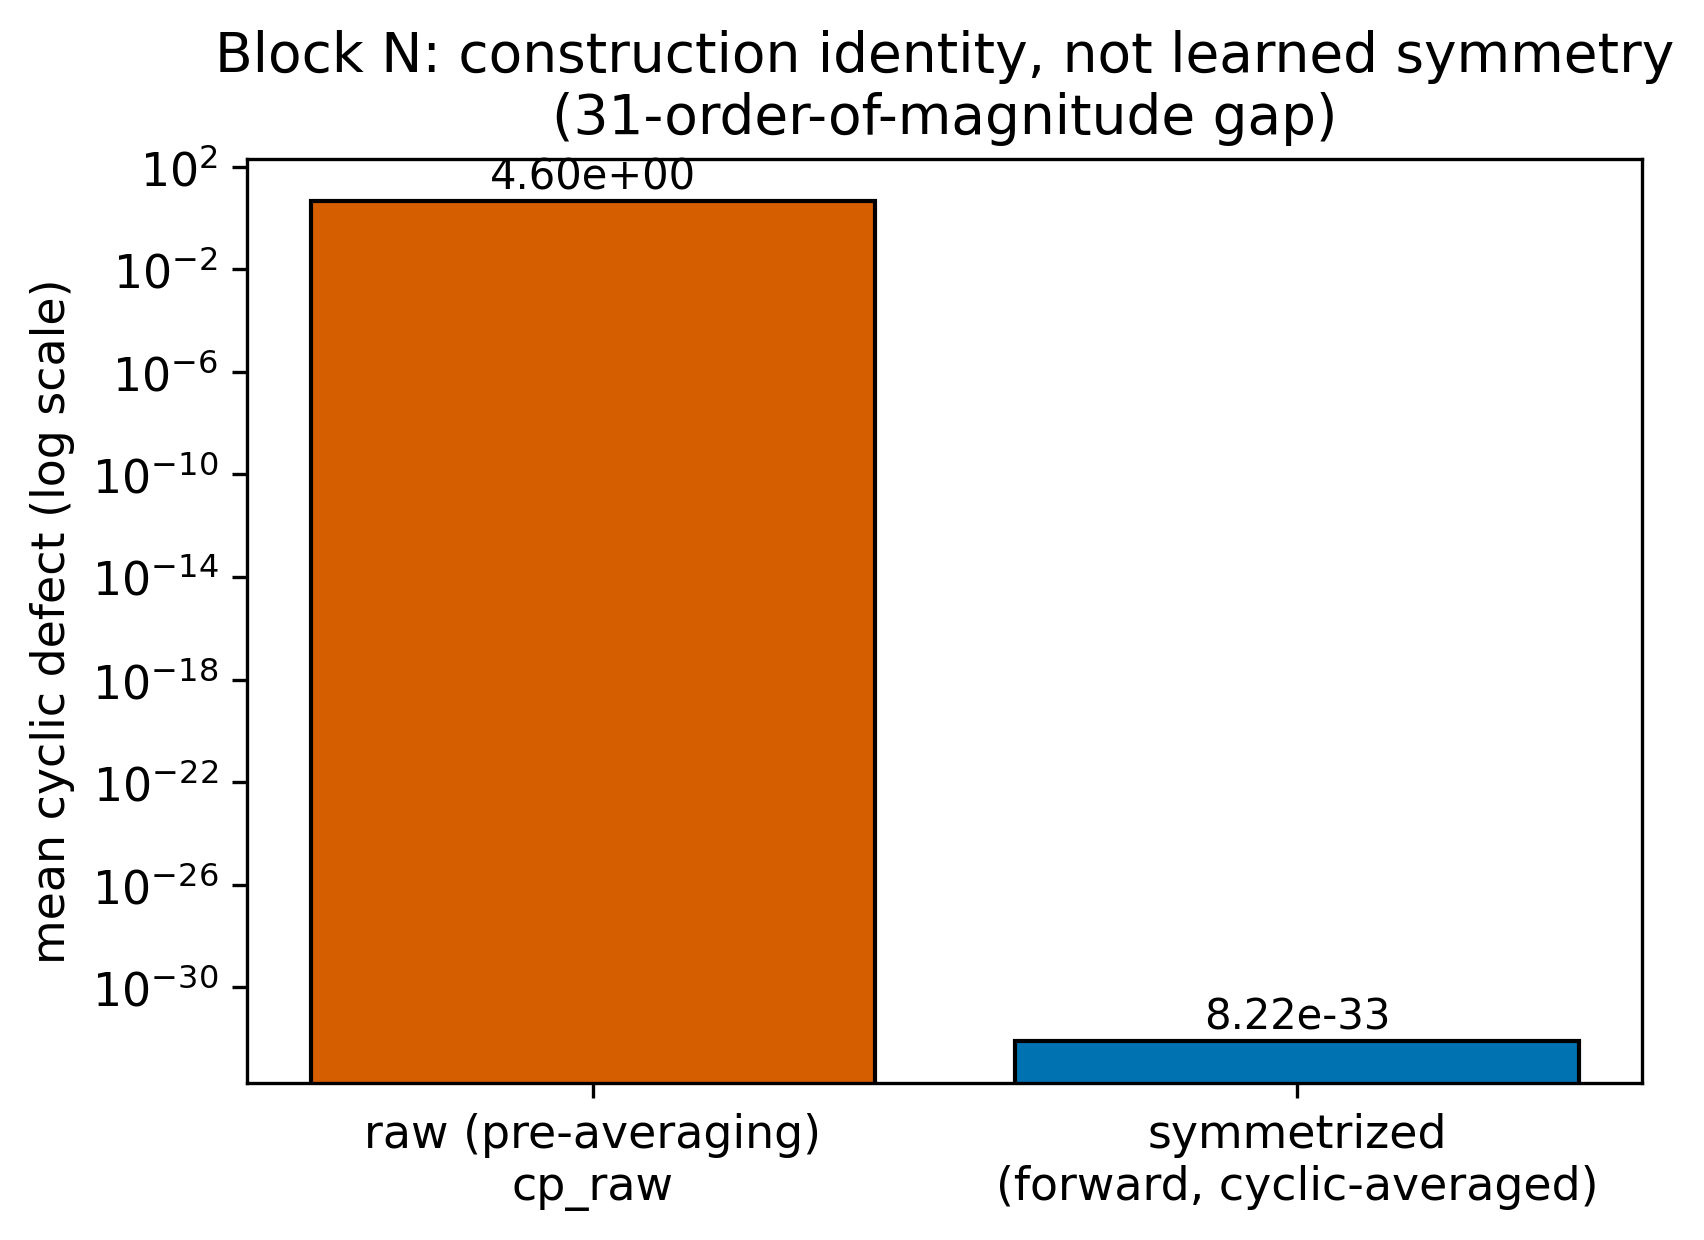
\includegraphics[width=0.7\textwidth]{05_block_n_cyclic}
\caption{Block N: raw vs.\ symmetrized cyclic defect on a log scale. The
symmetrized bar sits at machine-precision zero ($8.2\times10^{-33}$,
displayed at a floor for visibility) --- a construction identity, not
learned symmetry.}
\end{figure}

\begin{figure}[h]
\centering
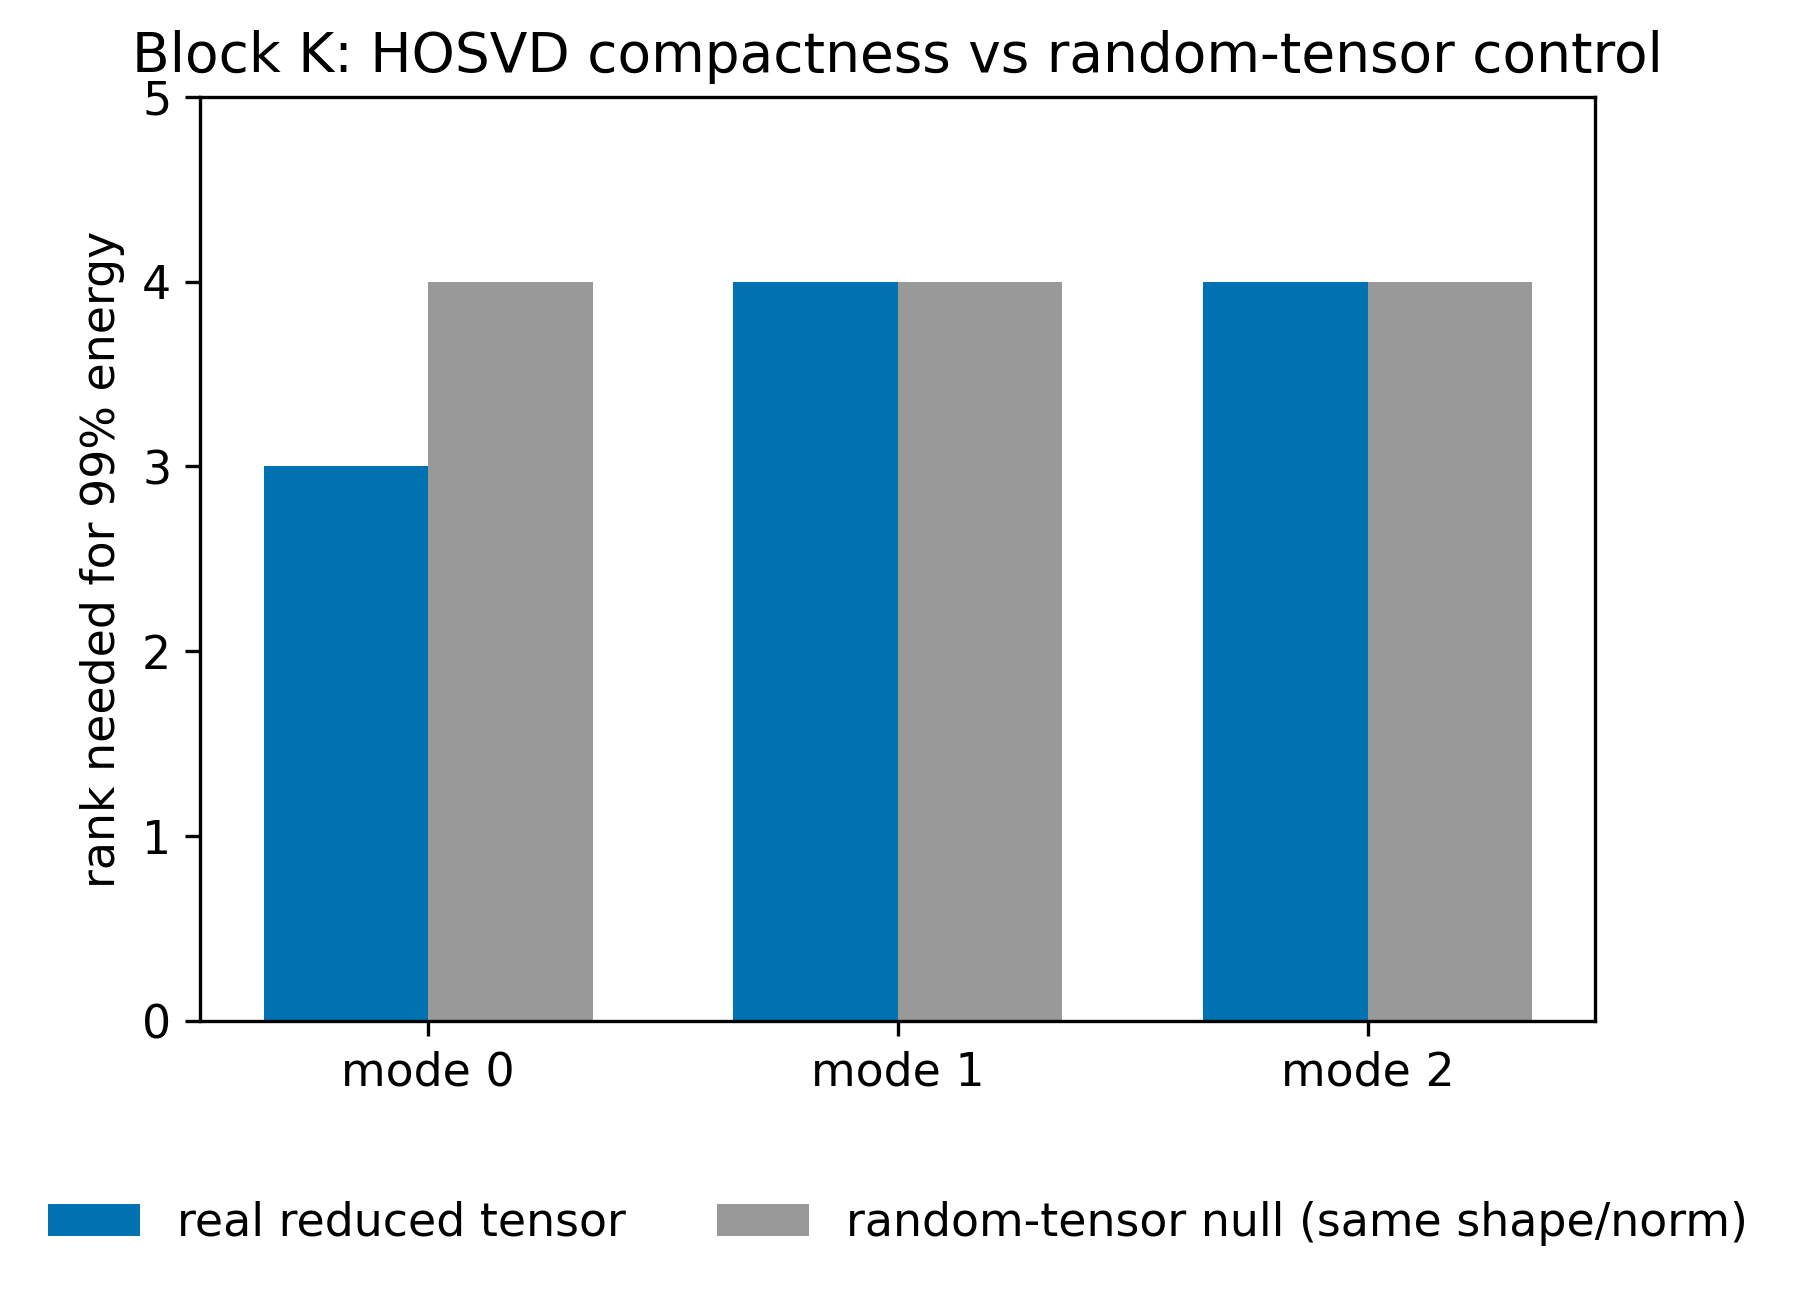
\includegraphics[width=0.7\textwidth]{06_block_k_hosvd}
\caption{Block K: real reduced tensor vs.\ a norm-matched random-tensor
null, per mode. The real tensor is only more compact than the random null
in mode 0; modes 1 and 2 tie it exactly.}
\end{figure}

\begin{figure}[h]
\centering
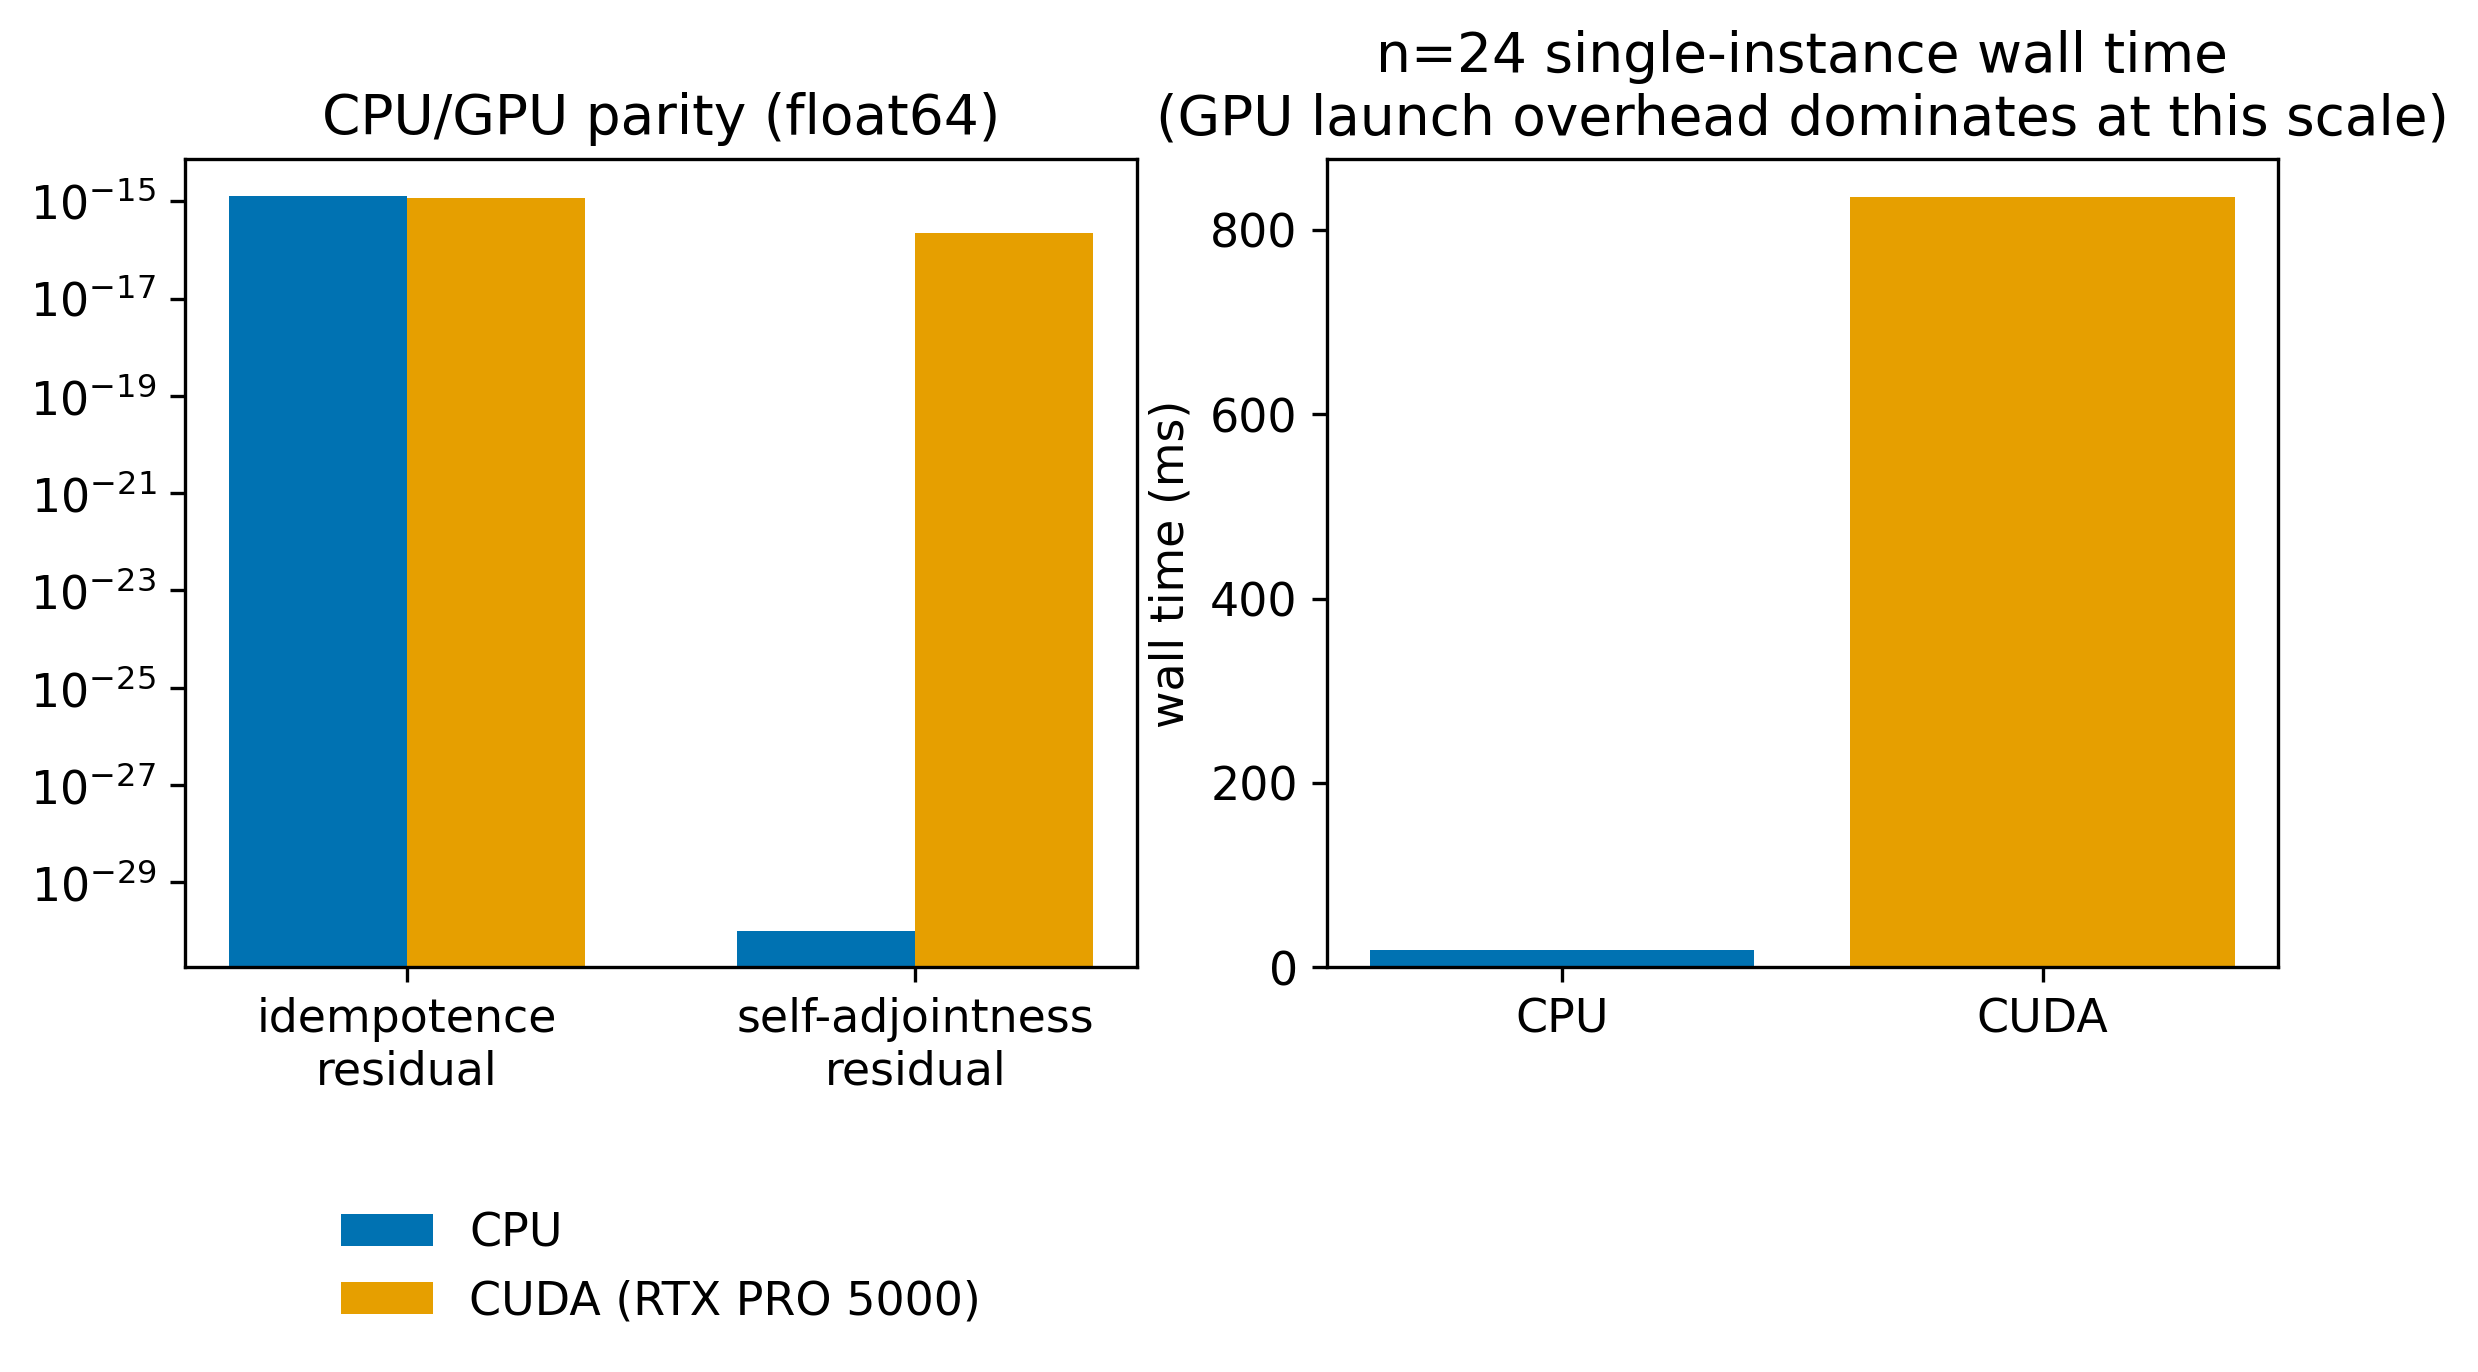
\includegraphics[width=0.95\textwidth]{07_hardware_parity}
\caption{Left: CPU vs.\ CUDA (RTX PRO 5000 Blackwell) parity for two
projector residuals, float64, TF32 disabled --- both at the numerical
noise floor on both devices. Right: wall time at $n=24$; GPU kernel-launch
overhead dominates at this small scale, an honest negative scaling result
for this problem size.}
\end{figure}

\begin{figure}[h]
\centering
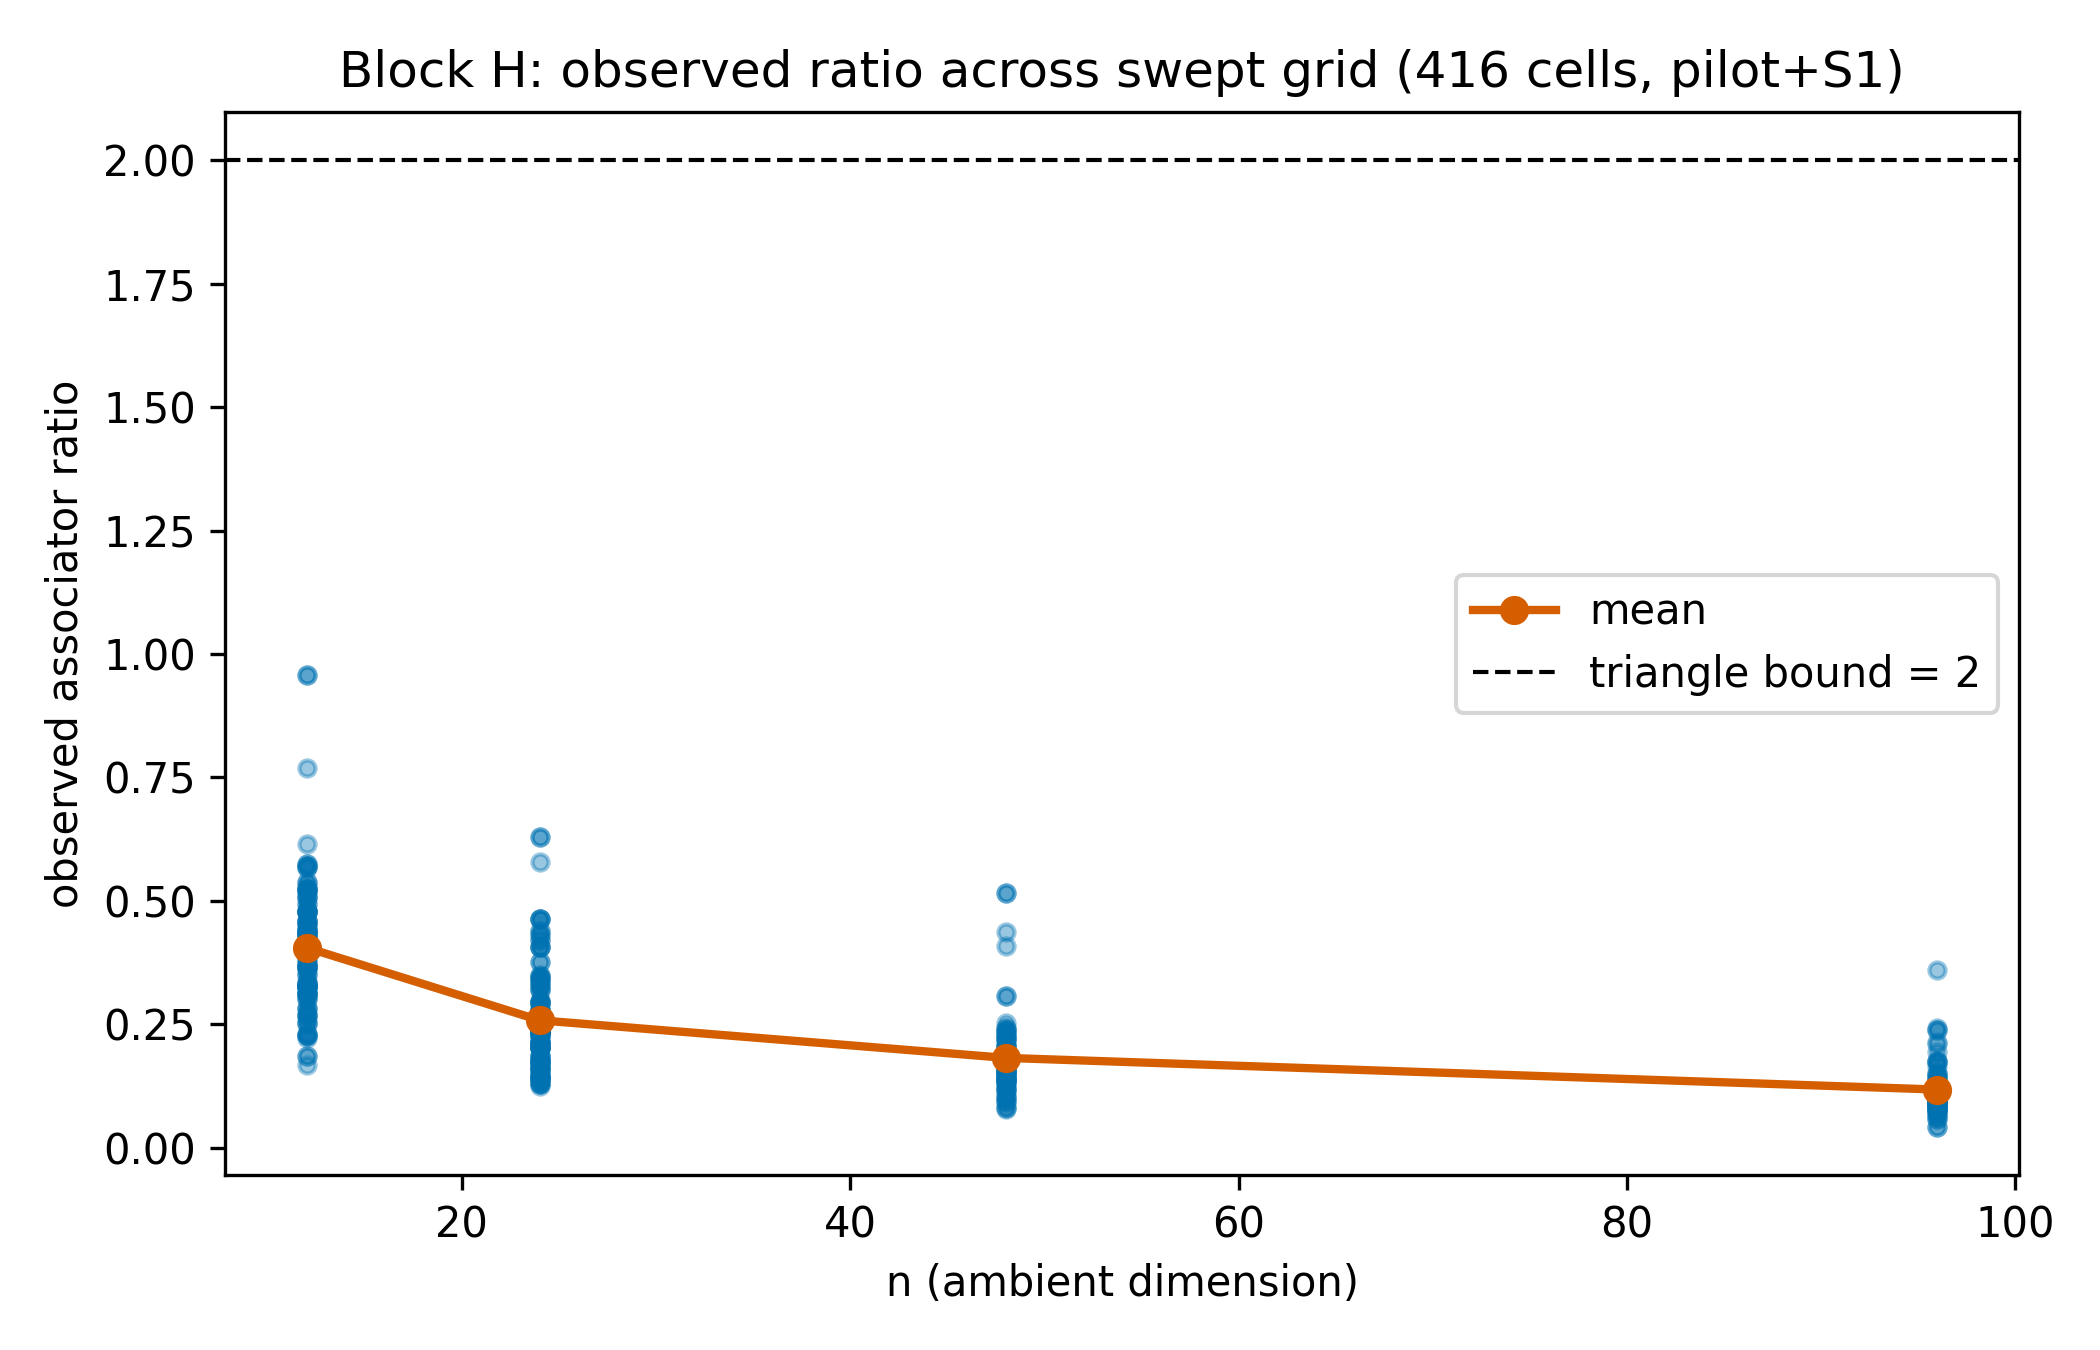
\includegraphics[width=0.85\textwidth]{08_block_h_swept_grid}
\caption{Block H's observed associator ratio across the full 416-cell
pilot+S1 sweep (arity $\in\{3,4\}$, rank $\in\{3,6\}$, cp-rank
$\in\{4,8\}$, 3--5 seeds, $n\in\{12,24,48,96\}$) --- the swept-grid
surface the original atlas explicitly listed as missing. A new pattern
visible only at this scale: the mean ratio \emph{decreases} monotonically
with $n$ (0.40 at $n{=}12$ to 0.11 at $n{=}96$), moving further from the
triangle bound of 2 as ambient dimension grows, not closer --- the
single-configuration result in Figure~4 ($n{=}16$, ratio 0.452) sits
consistently with this trend, not as an outlier.}
\end{figure}

\begin{figure}[h]
\centering
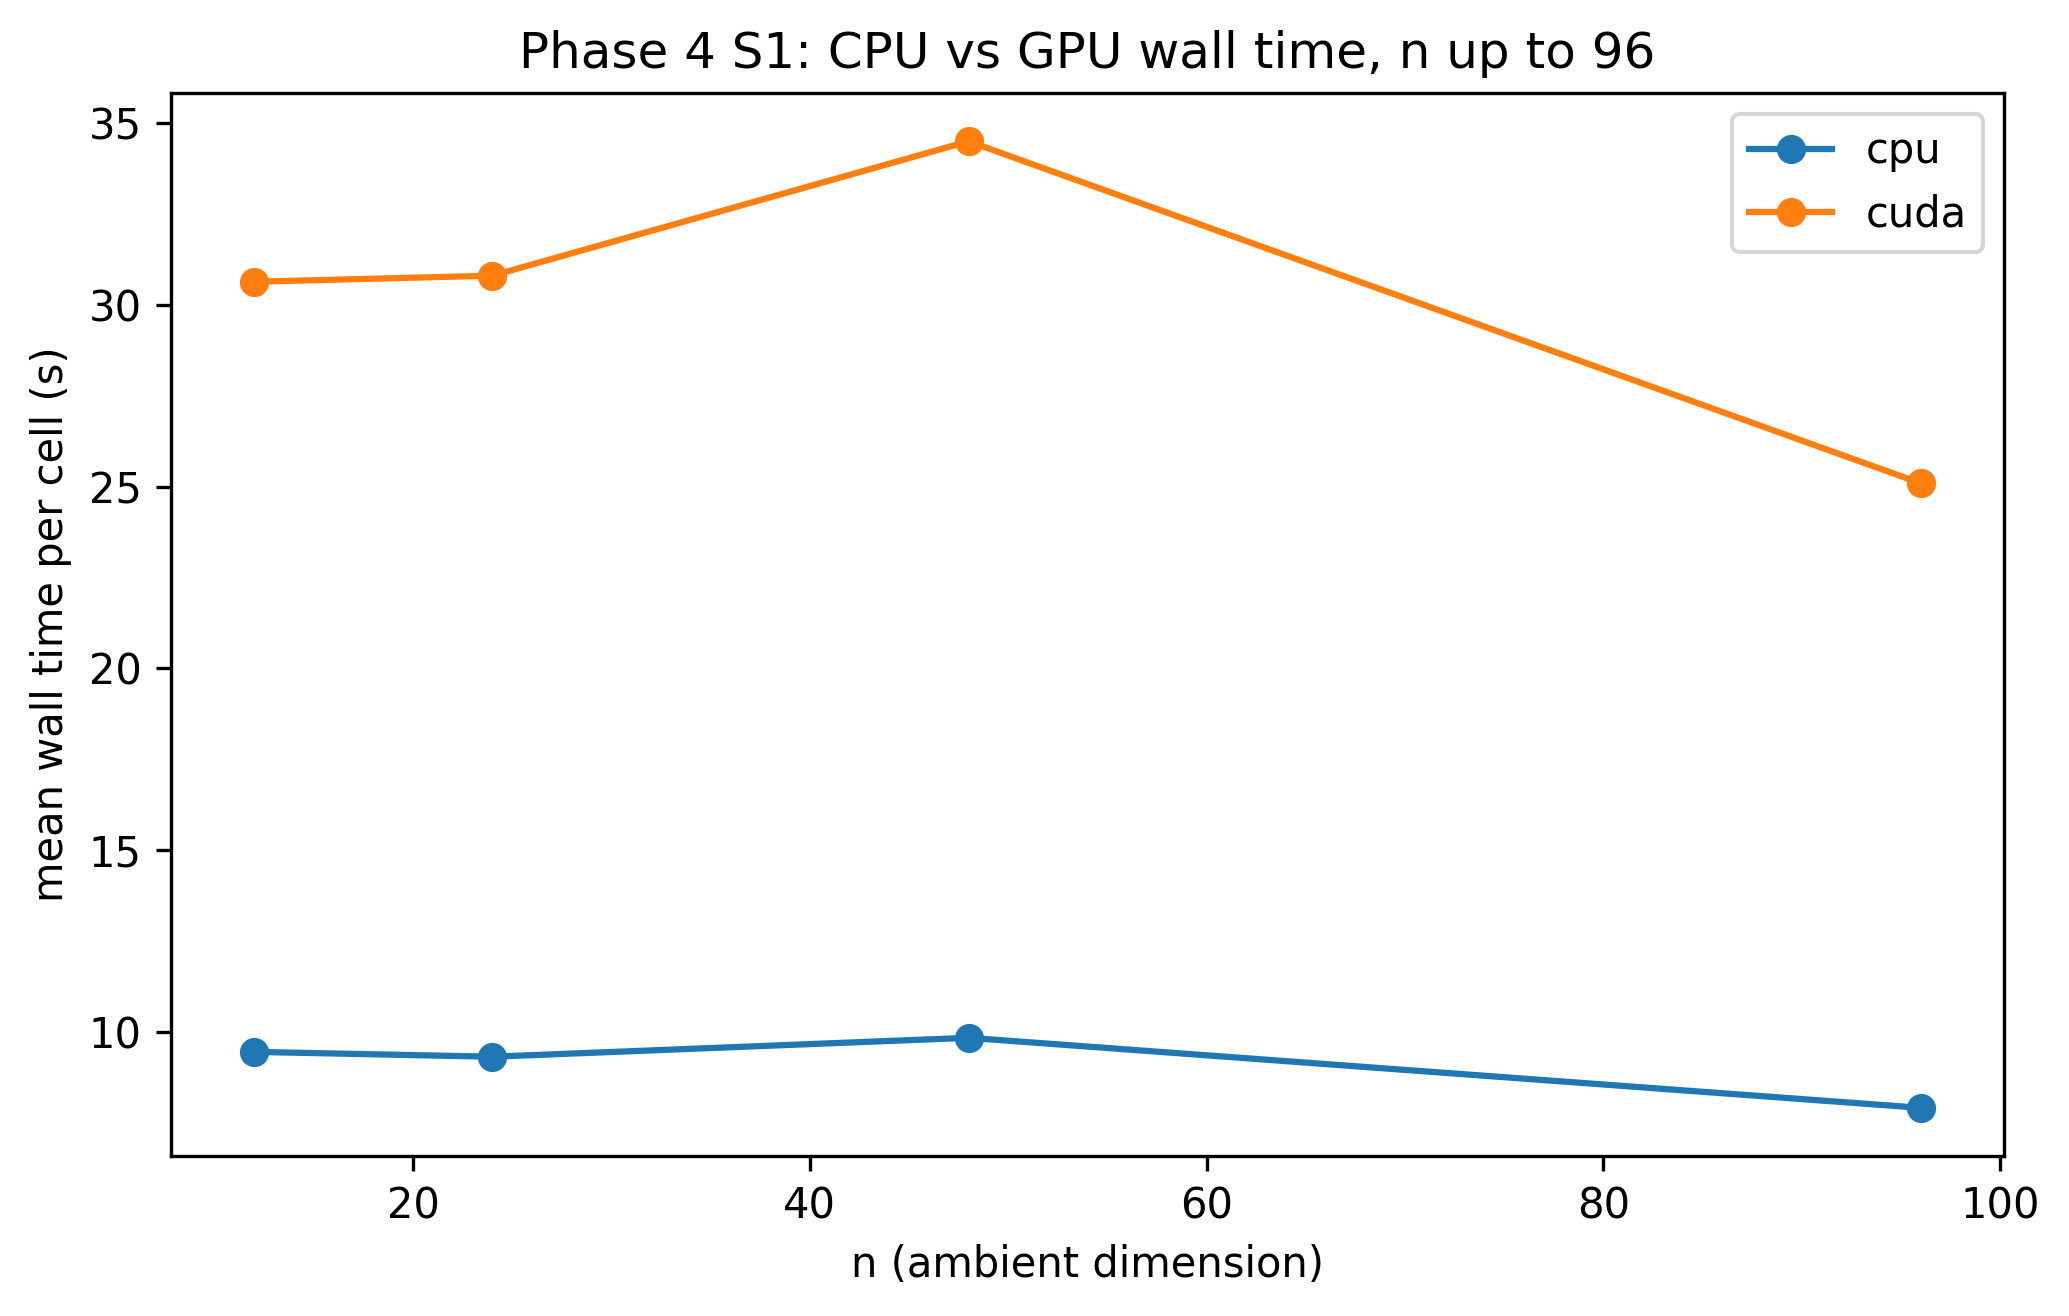
\includegraphics[width=0.85\textwidth]{09_gpu_cpu_scaling}
\caption{CPU vs.\ GPU mean wall time per cell across
$n\in\{12,24,48,96\}$, 320 cells (Stage S1 broad screening). Directly
answers the scaling question Figure~7's single-dimension comparison left
open: GPU never overtakes CPU anywhere in this range, a stable
$3.2\times$--$3.5\times$ CPU advantage throughout rather than a
small-$n$-only artifact.}
\end{figure}

\section{What is intentionally not included here}
\label{sec:missing}
\begin{itemize}
\item Topology/dimension/eta phase diagrams and the $k$ vs.\ $k{-}1$
  theorem geometry --- these belong to Track T, explicitly deferred.
\item A full gauge-orbit diagram (beyond the single degenerate-eigenspace
  example in \texttt{BLOCK\_L\_FINDINGS.md}) and a GJI permutation/sign
  atlas --- not generated this pass; the underlying data (permutation
  mutation test, degenerate-eigenspace construction) exists in
  \texttt{spectral/certification\_v18/blocks/} but was not turned into a
  dedicated figure.
\item Closure adversarial-maxima surfaces across a swept parameter grid
  --- Figure~8 closes this gap for block H specifically (associator);
  block G's closure defect was not swept the same way this pass.
\item Precision/CPU-GPU parity across multiple blocks and dimensions ---
  Figure~9 closes this for blocks A/G/H/N across $n\in\{12,24,48,96\}$;
  blocks B, C, D, E, F, I, J, K, L, M remain CPU-only and untested for
  this question (no \texttt{device} parameter was added to their report
  functions this pass).
\end{itemize}

\end{document}
